% This work is made available under the terms of the
% Creative Commons Attribution-ShareAlike 4.0 license,
% http://creativecommons.org/licenses/by-sa/4.0/.

\chapter{Tools}

\section{WEKA Append datasets}

If you have datasets with the same structure, i.e., exactly the same
attributes, then you can use the \textit{Append datasets} tool to combine
them into a single, large dataset.

The screenshot in Figure \ref{dataset-compatibility} shows the wizard
interface that guides you through the process.

\begin{figure}[htb]
  \centering
  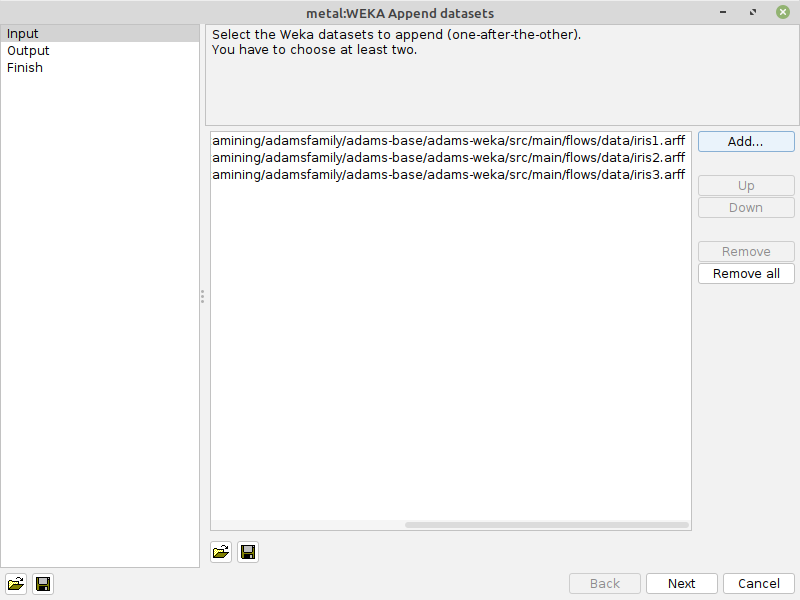
\includegraphics[width=12.0cm]{images/append_datasets.png}
  \caption{Appending datasets wizard.}
  \label{append_datasets}
\end{figure}

\clearpage
\section{WEKA Batch-filter datasets}

Training and test set are required to have exactly the same structure
in WEKA. If you need to apply a pre-processing filter to both of the
files, it is recommended to use \textit{batch-filtering}. This will
ensure that any statistics that get calculated based on the first
dataset, get applied to second file as well. An example for this is
the dictionary of the \textit{StringToWordVector}: the same word
dictionary needs to be applied to the second file, in order to generate
the same attributes. However, one usually has to resort to the command-line
in order to achieve this, which is rather tedious.

The \textit{Batch-filter datasets} wizard allows you to perform the
batch-filtering conveniently through the GUI:
\begin{tight_itemize}
  \item Select the datasets to filter (see \ref{batchfilter_datasets1})
  \item Configure the filter (see \ref{batchfilter_datasets2})
  \item Select the output directory (see \ref{batchfilter_datasets3})
  \item Info dialog after filtering (see \ref{batchfilter_datasets4})
\end{tight_itemize}

\begin{figure}[htb]
  \centering
  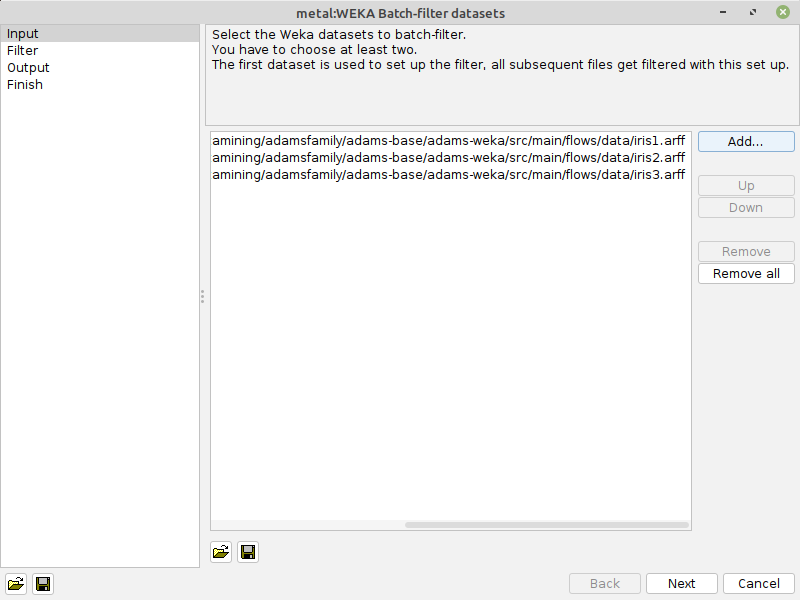
\includegraphics[width=12.0cm]{images/batchfilter_datasets1.png}
  \caption{Selecting input files for batch-filtering.}
  \label{batchfilter_datasets1}
\end{figure}

\begin{figure}[htb]
  \centering
  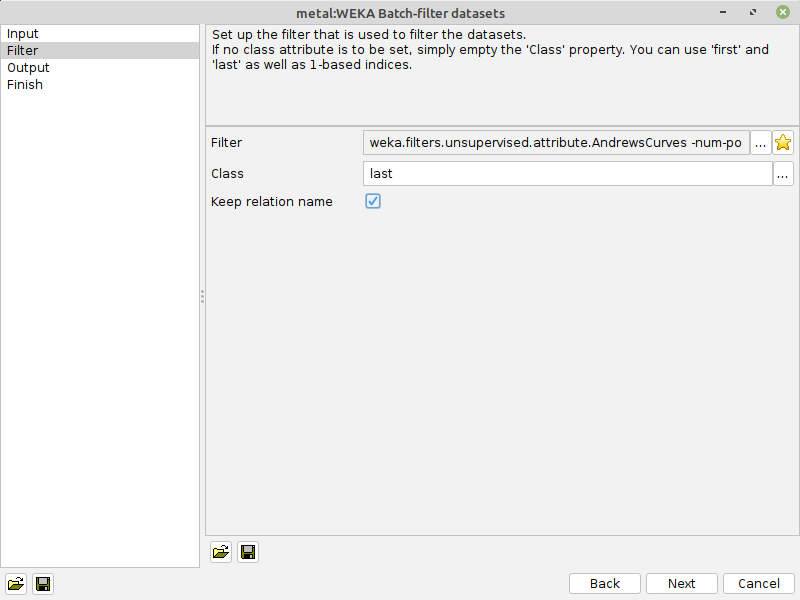
\includegraphics[width=12.0cm]{images/batchfilter_datasets2.png}
  \caption{Configuring the filter.}
  \label{batchfilter_datasets2}
\end{figure}

\begin{figure}[htb]
  \centering
  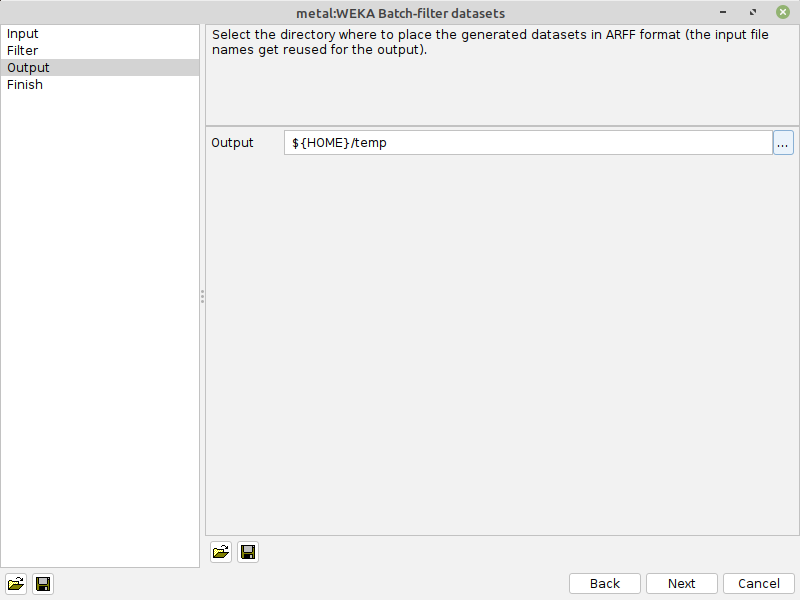
\includegraphics[width=12.0cm]{images/batchfilter_datasets3.png}
  \caption{Selecting the output directory for the filtered datasets.}
  \label{batchfilter_datasets3}
\end{figure}

\begin{figure}[htb]
  \centering
  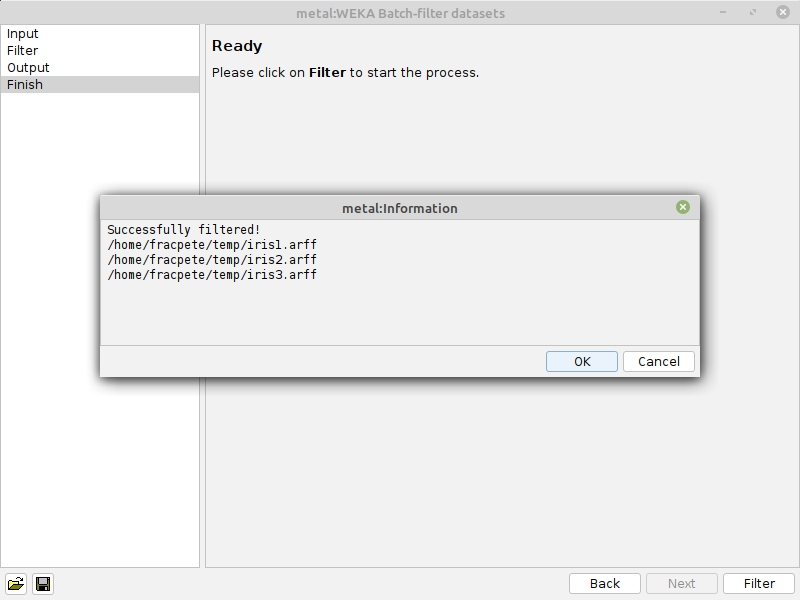
\includegraphics[width=12.0cm]{images/batchfilter_datasets4.png}
  \caption{The dialog when batch-filtering was successful.}
  \label{batchfilter_datasets4}
\end{figure}

\clearpage
\section{WEKA Dataset compatibility}

WEKA requires training and test sets to have the same structure, down to the
same name and order of nominal labels. Rather than relying on the error message
in the Explorer, you can use the \textit{Dataset compatibility} tool to 
quickly check whether two or more datasets are actually compatible.

The screenshot in Figure \ref{dataset-compatibility} shows the output when
comparing two datases, one being the original \textit{anneal} UCI dataset
and the other one a transformed version.

\begin{figure}[htb]
  \centering
  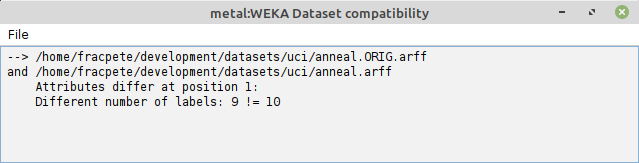
\includegraphics[width=12.0cm]{images/dataset-compatibility.png}
  \caption{Compatibility output for two datasets.}
  \label{dataset-compatibility}
\end{figure}

\clearpage
\section{WEKA Make compatible datasets}
When dealing with data across multiple spreadsheets, e.g., training, test
and validation set, then it can happen that these datasets are not compatible
in the strict Weka sense.

The \textit{Make compatible datasets} wizard allows you to turn spreadsheets
into compatible ARFF files:
\begin{tight_itemize}
  \item Select the datasets to make compatible (see \ref{makecompatible1})
  \item Configure how the datasets are being read (see \ref{merge_datasets2})
  \item Select the output directory for the compatible ARFF files (see \ref{merge_datasets3})
  \item Info dialog after processing the datasets (see \ref{merge_datasets4})
\end{tight_itemize}

\begin{figure}[htb]
  \centering
  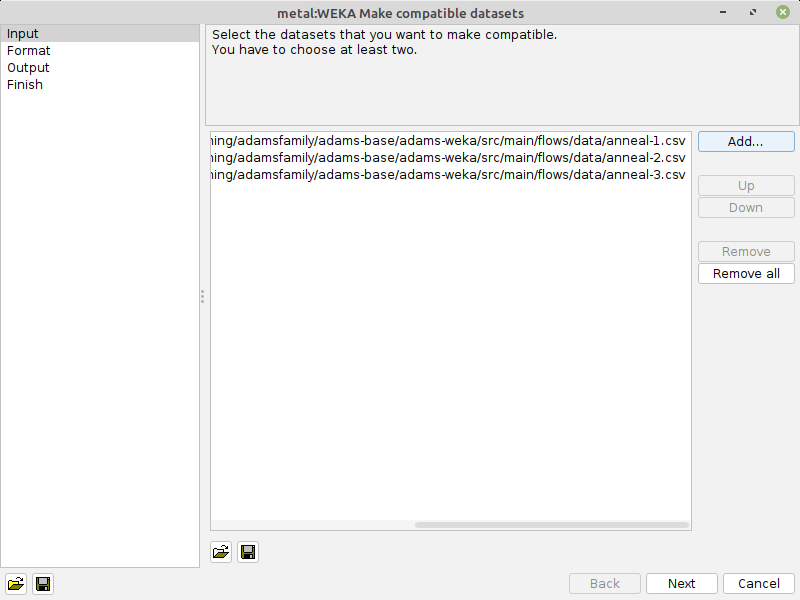
\includegraphics[width=12.0cm]{images/makecompatible1.png}
  \caption{Selecting input files for making compatible datasets.}
  \label{makecompatible1}
\end{figure}

\begin{figure}[htb]
  \centering
  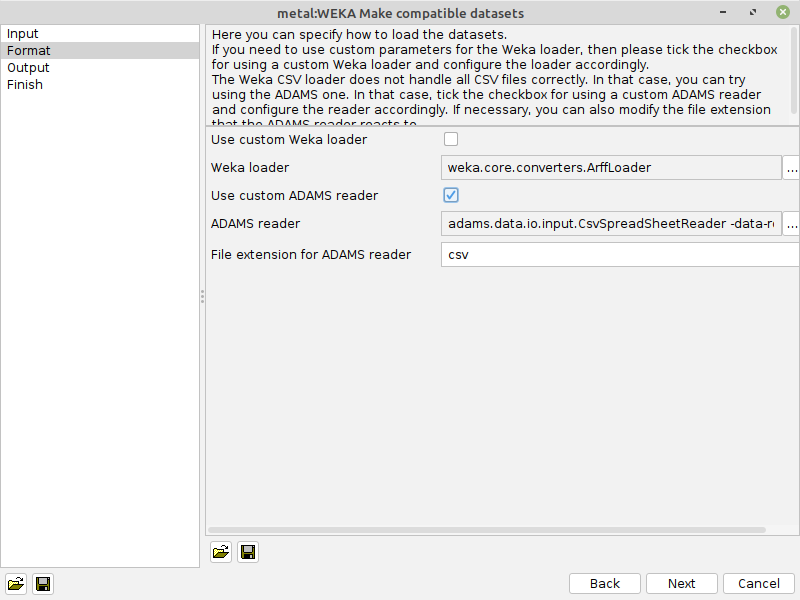
\includegraphics[width=12.0cm]{images/makecompatible2.png}
  \caption{Configuring the readers for the datasets.}
  \label{makecompatible2}
\end{figure}

\begin{figure}[htb]
  \centering
  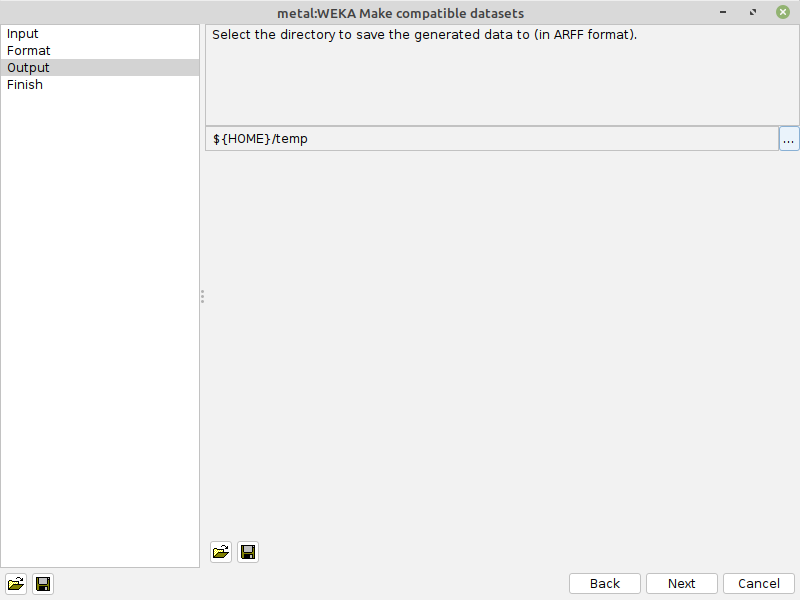
\includegraphics[width=12.0cm]{images/makecompatible3.png}
  \caption{Selecting the output directory for the compatible ARFF files.}
  \label{makecompatible3}
\end{figure}

\begin{figure}[htb]
  \centering
  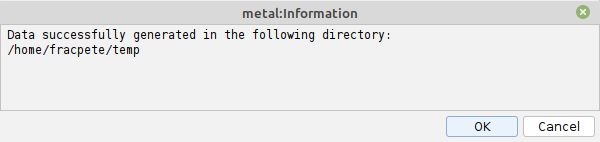
\includegraphics[width=8.0cm]{images/makecompatible4.png}
  \caption{The dialog when dataset generation was successful.}
  \label{makecompatible4}
\end{figure}

\clearpage
\section{WEKA Merge datasets}
The process of adding reference data to a dataset or performing
\textit{data fusion}\footnote{\url{https://en.wikipedia.org/wiki/Data_fusion}{}},
can be quite often a manual process, copy/pasting datasets in a spreadsheet
application.

The \textit{Merge datasets} wizard allows you to perform the
process of combining datasets side-by-side conveniently in the GUI:
\begin{tight_itemize}
  \item Select the datasets to merge (see \ref{merge_datasets1})
  \item Configure the merge (see \ref{merge_datasets2})
  \item Select the output file (see \ref{merge_datasets3})
  \item Info dialog after merging (see \ref{merge_datasets4})
\end{tight_itemize}
Figure \ref{merge_datasets-output} shows an example of a merged file.

\begin{figure}[htb]
  \centering
  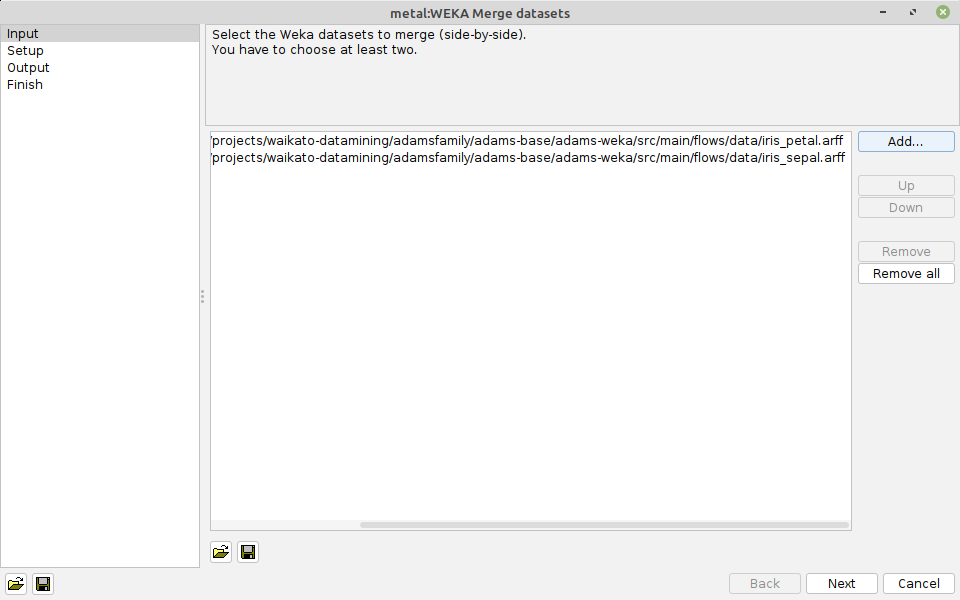
\includegraphics[width=12.0cm]{images/merge_datasets1.png}
  \caption{Selecting input files for merging.}
  \label{merge_datasets1}
\end{figure}

\begin{figure}[htb]
  \centering
  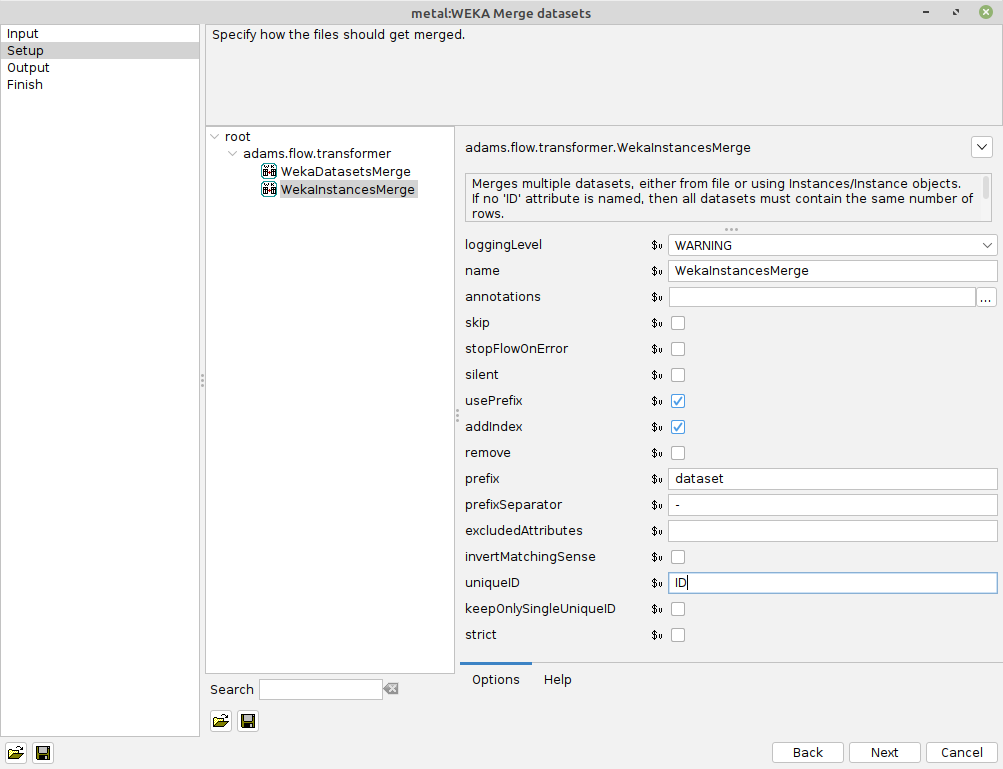
\includegraphics[width=12.0cm]{images/merge_datasets2.png}
  \caption{Configuring the merge.}
  \label{merge_datasets2}
\end{figure}

\begin{figure}[htb]
  \centering
  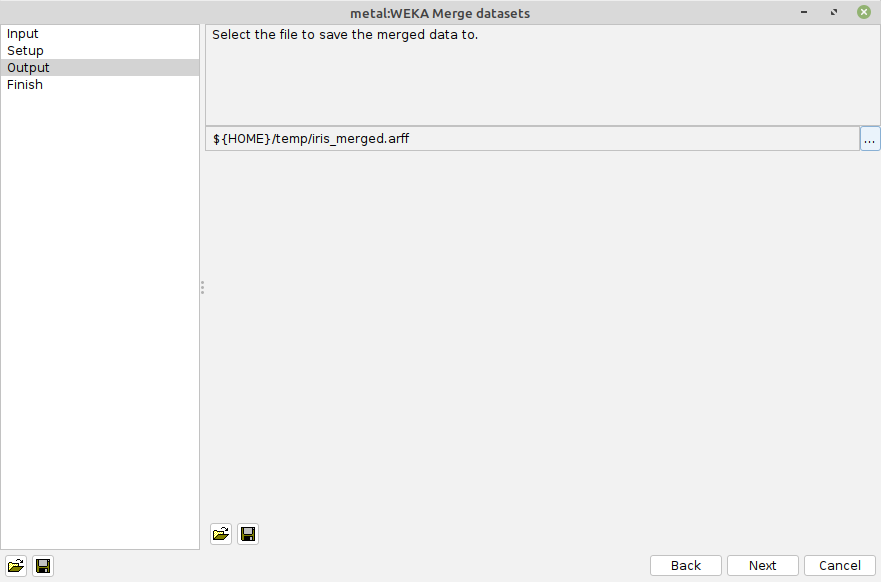
\includegraphics[width=12.0cm]{images/merge_datasets3.png}
  \caption{Selecting the file to save the merged dataset to.}
  \label{merge_datasets3}
\end{figure}

\begin{figure}[htb]
  \centering
  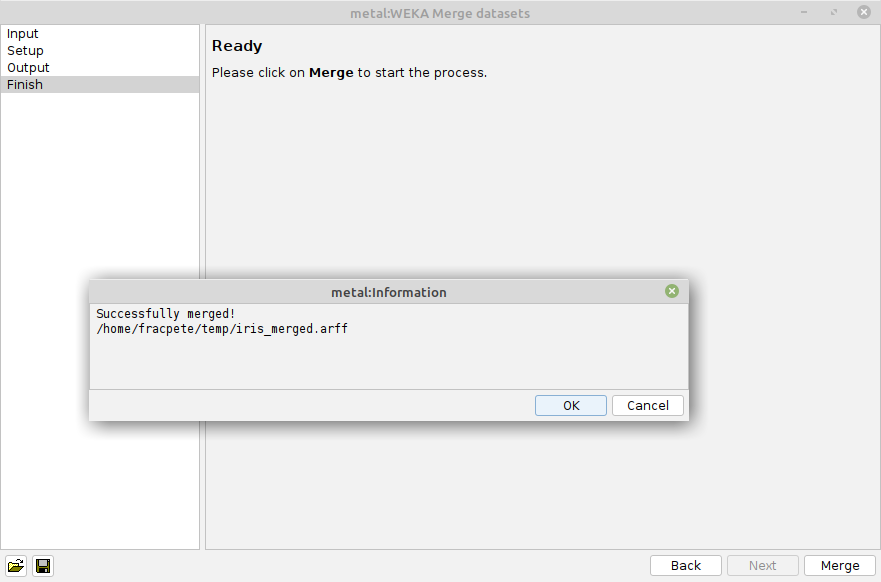
\includegraphics[width=12.0cm]{images/merge_datasets4.png}
  \caption{The dialog when merging was successful.}
  \label{merge_datasets4}
\end{figure}

\begin{figure}[htb]
  \centering
  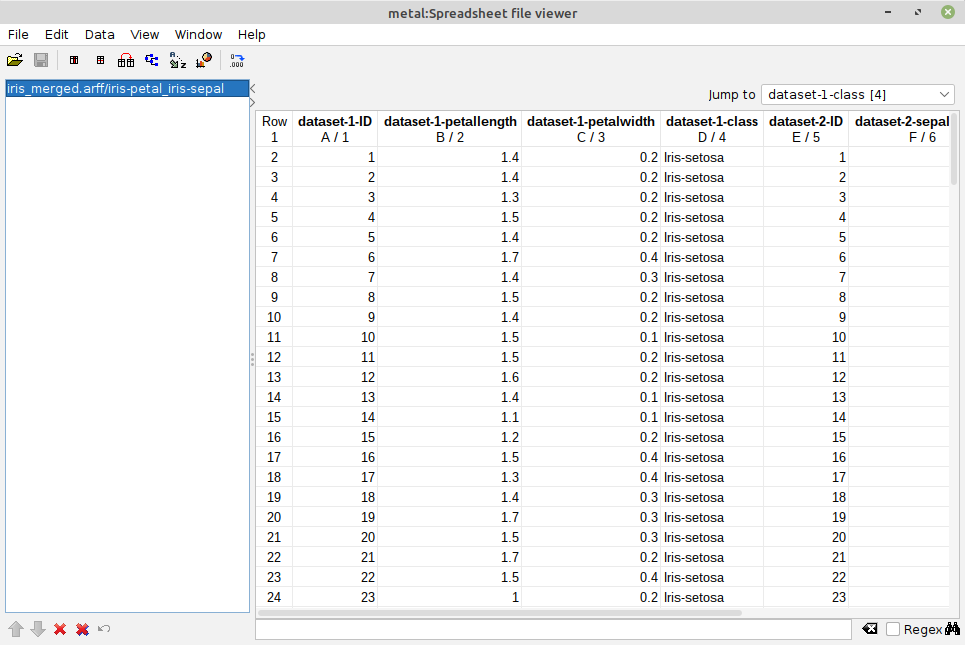
\includegraphics[width=12.0cm]{images/merge_datasets-output.png}
  \caption{The merged dataset.}
  \label{merge_datasets-output}
\end{figure}
